\documentclass[12pt]{mypackage}

% sans serif font:
%\usepackage{cmbright}
%\usepackage{sfmath}
%\usepackage{bbold} %better blackboard bold

%serif font + different blackboard bold for serif font
%\pgfplotsset{compat=newest}
\usepackage{newpxtext,eulerpx}
\renewcommand*{\mathbb}[1]{\varmathbb{#1}}
\pagestyle{fancy}
\fancyhf{}
\rhead{Avinash Iyer}
\lhead{Ordinary Differential Equations: Homework 1}

\setcounter{secnumdepth}{0}

\begin{document}
\section{Part 1}%
\subsection{1.1, Problem 2}%
The equilibrium solution occurs when $\frac{dy}{dt} = 0$, meaning
\begin{align*}
  0 &= \frac{\left(t^2 - 1\right)\left(y^2 - 2\right)}{y^2 - 4}\\
  y^2 - 2 &= 0\\
  y(t) &= \sqrt{2}\\
  y(t) &= -\sqrt{2}.
\end{align*}
\subsection{1.1, Problem 3}%
\begin{enumerate}[(a)]
  \item When $P = 0$ or $P = 230$, the population is in equilibrium.
  \item If $P$ is between $0$ and $230$, the population is increasing.
  \item If $P$ is greater than $230$ or less than $0$, the population is decreasing.
\end{enumerate}
\subsection{1.1, Problem 13}%
Learning occurs most rapidly when $L = 0$.
\subsection{1.1, Problem 14}%
\begin{enumerate}[(a)]
  \item The student who knows one half of the list at $t=0$ learns at a slower rate than the student who knows none of the list.
  \item The student who starts out knowing none of the list will never catch up to the student who starts out knowing one half of the list because solutions to initial value problems cannot intersect.
\end{enumerate}
\section{Part 2}%
\subsection{1.2, Problem 1}%
\begin{enumerate}[(a)]
  \item Glen and Bob are correct; taking $y(t) = 2t+1$, we see that $\frac{dy}{dt} = 2 = \frac{2t+2}{t+1}$, and similarly, taking $y(t) = t$, we see $\frac{dy}{dt} = 1 = \frac{t+1}{t+1}$.
  \item The solution of $y(t) = t$ should be immediately obvious from separation of variables.
\end{enumerate}
\subsection{1.2, Problem 2}%
Substituting $y=e^{2t}$, we find that $t = \frac{1}{2}\ln y$, meaning we have $y(t) = e^{2t}$ is a solution to $\frac{dy}{dt} = 2y - t + \frac{1}{2}\ln y$.
\subsection{1.2, Problem 3}%
The derivative $\frac{dy}{dt}$ for $y(t) = e^{t^3}$ is $3t^2 e^{t^3}$. Substituting $y = e^{t^3}$, we find that $y(t) = e^{t^3}$ is a solution to the equation $\frac{dy}{dt} = 3t^2y$.
\subsection{1.2, Problem 27}%
Since $y(t) = 0$ is an equilibrium solution for $\frac{dy}{dt} = -y^2$, and $y(0) = 0$, we have that $y(t) = 0$ solves the initial value problem.
\subsection{1.2, Problem 32}%
\begin{align*}
  \frac{dy}{dt} &= ty^2 + 2y^2\\
  \frac{dy}{dt} &= y^2\left(t+2\right)\\
  \frac{1}{y^2}\:dy &= \frac{1}{t+2}\:dt\\
  \int_{}^{} \frac{1}{y^2}\:dy &= \int_{}^{} \frac{1}{t+2}\:dt\\
  -\frac{1}{y} &= \ln\left\vert t+2 \right\vert + C_1\\
  \frac{1}{y} &= C  - \ln \left\vert t+2 \right\vert\\
  y &= \frac{1}{C - \ln \left\vert t+2 \right\vert}.
\end{align*}
Including our initial value $y(0) = 1$, we find that
\begin{align*}
  C = 1 + \ln 2.
\end{align*}
Thus, the initial value problem has a solution of
\begin{align*}
  y(t) &= \frac{1}{\left(1 + \ln 2\right) - \ln \left\vert t+2 \right\vert}.
\end{align*}
\section{Part 3}%
\subsection{1.3, Problem 7}%
\begin{center}
  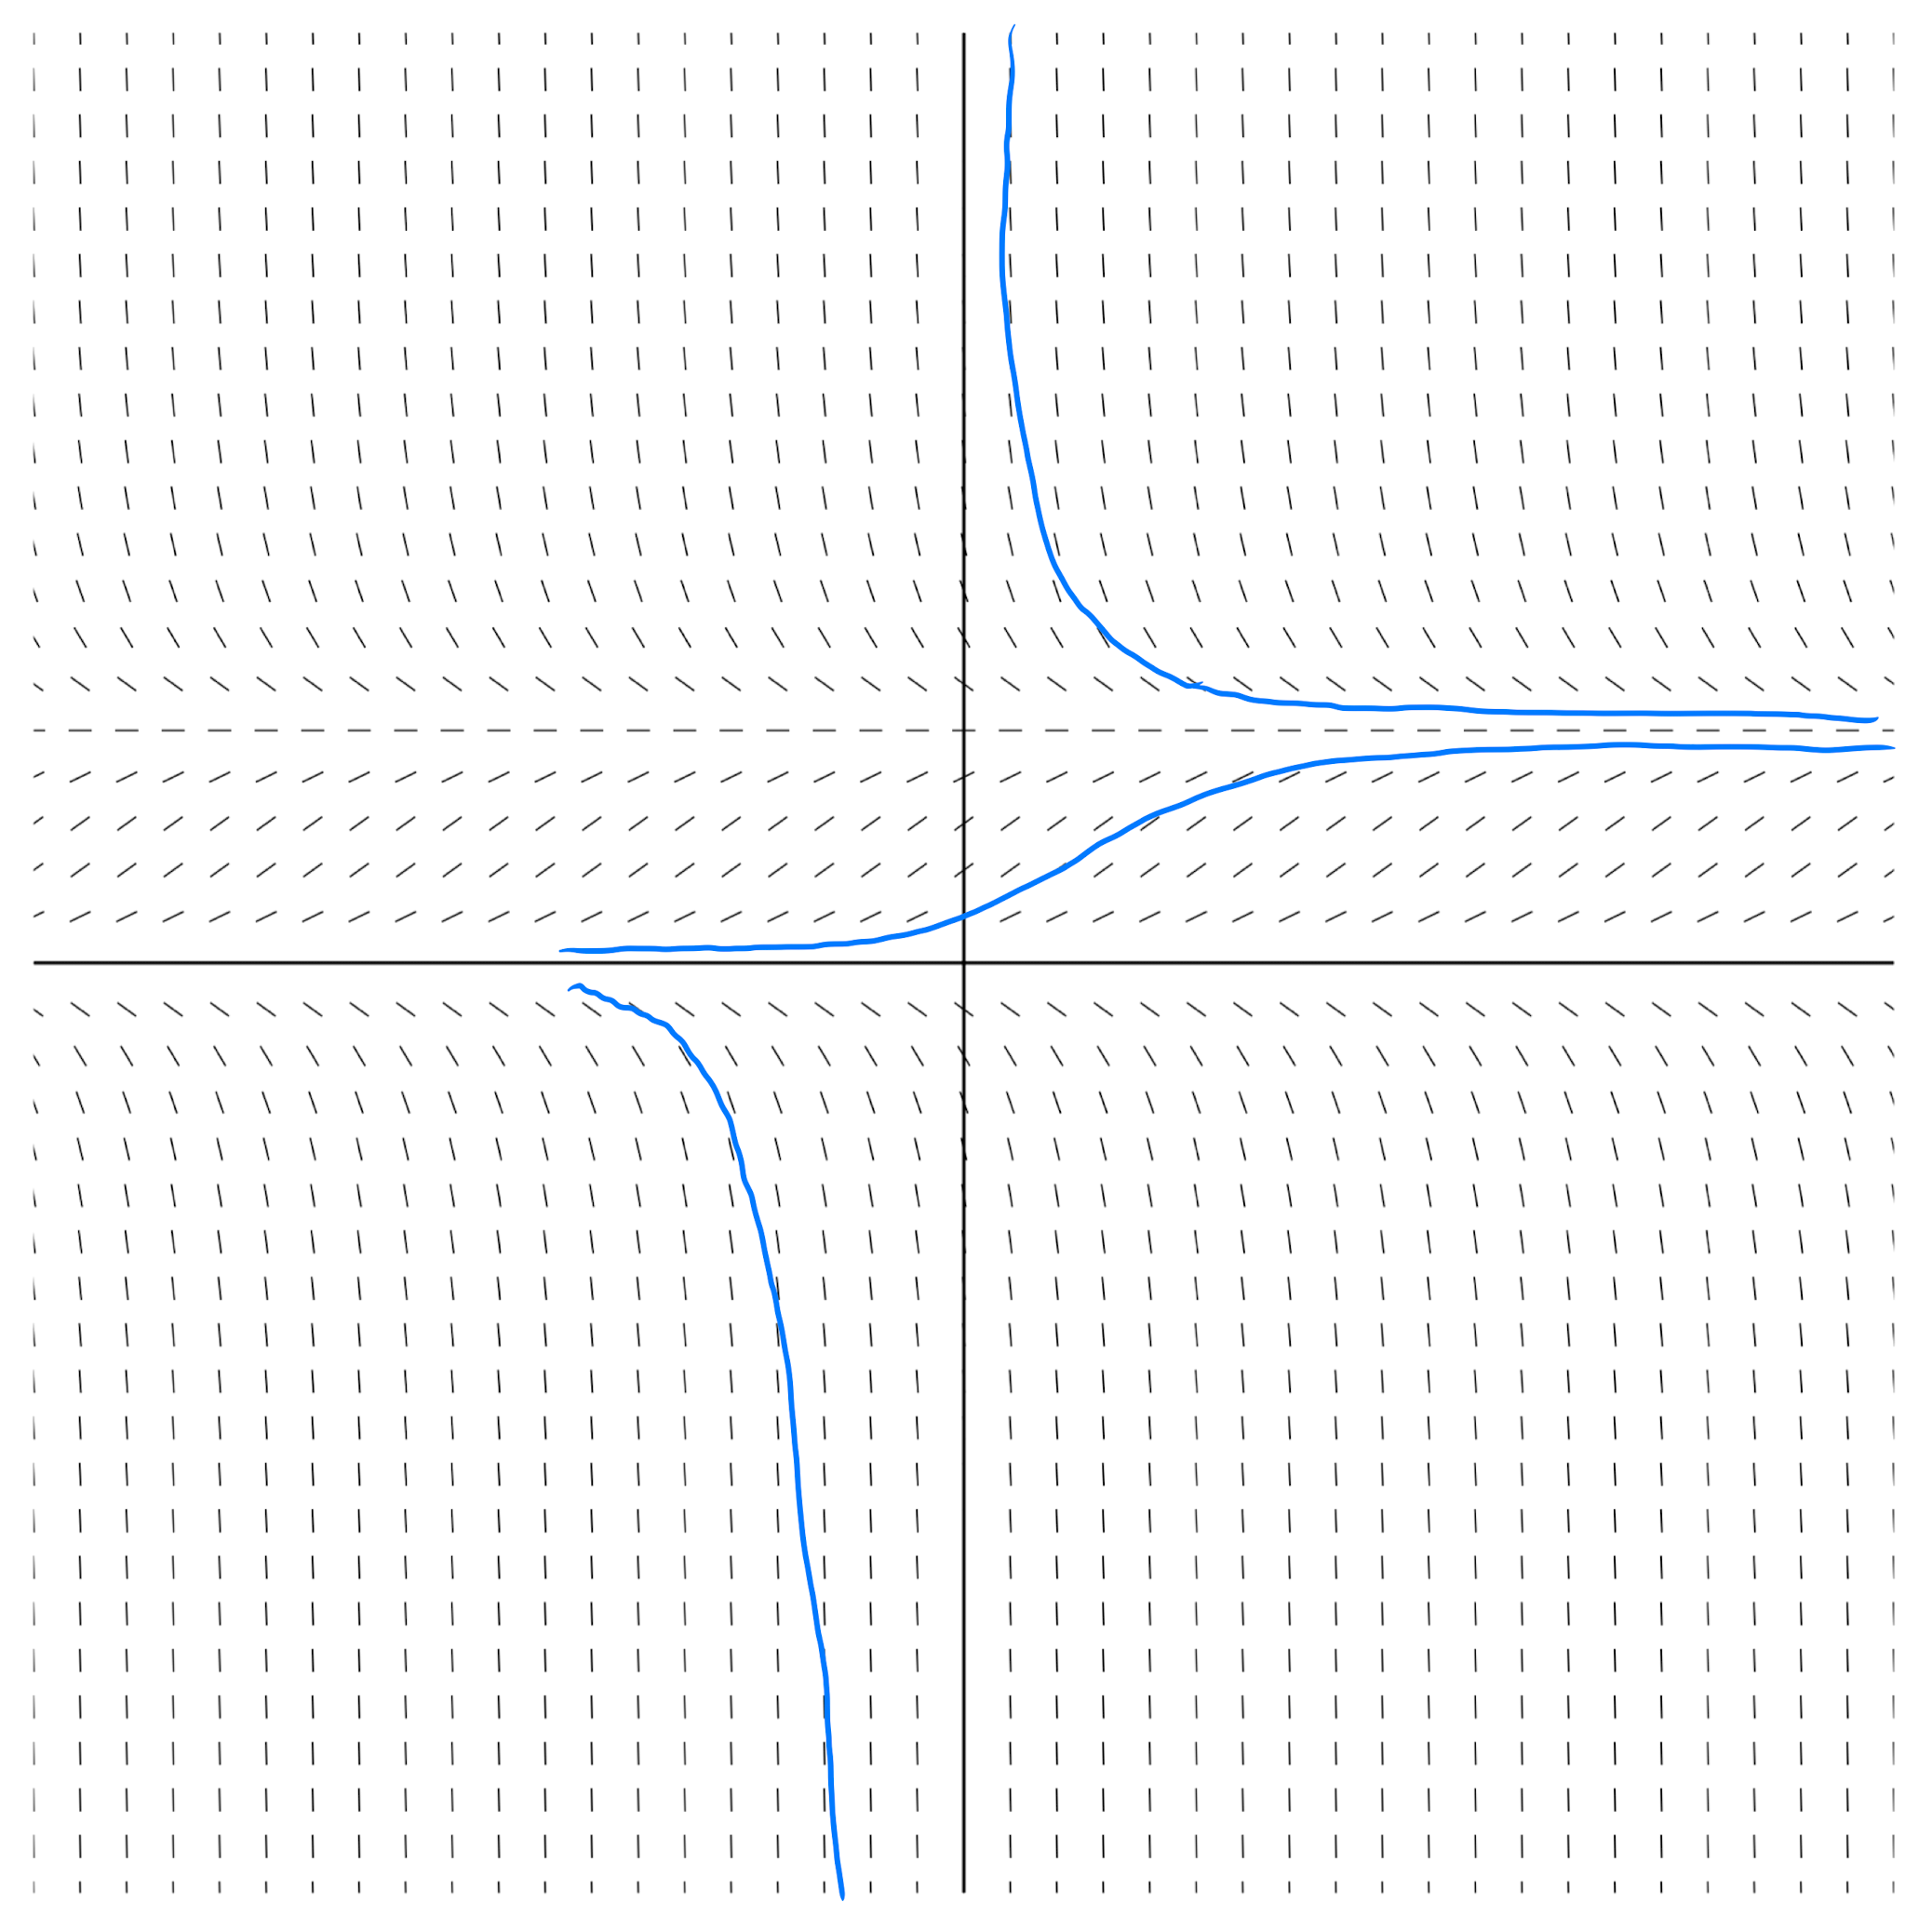
\includegraphics[width=7cm]{images/1_3_7.png}
\end{center}
For the solution with initial condition of $y(0) = 1/2$, the slope field suggests that, as $t$ increases, $y(t)$ approaches the equilibrium solution of $y(t) = -1$.
%\begin{center}
%  \begin{tikzpicture}[scale=2]
%    \begin{axis}[
%      view     = {0}{90},
%      domain   = -4:4,
%      y domain = -4:4,
%      samples  = 21,
%      xmax     = 4,
%      ymax     = 4,
%      ymin=-4,
%      xmin=-4,
%      axis lines*=center,
%      xtick={-4,-3,-2,-1,0,1,2,3,4},
%ytick={-4,-3,-2,-1,0,1,2,3,4},
%    ]
%    \addplot3 [gray, quiver={u={1}, v={(3*y(1-y))}, scale arrows=0.075,
%               every arrow/.append style={line width=0.5pt*\pgfplotspointmetatransformed/1000}}] (x,y,0);
%   % \addplot [thick, red] table [x=x, y=y] {\loadedtable};
%  \end{axis}
%  \end{tikzpicture}
%\end{center}
%\begin{align*}
%  \frac{dy}{dt} &= 3y\left(1-y\right).
%\end{align*}
\subsection{1.3, Problem 8}%
\begin{center}
  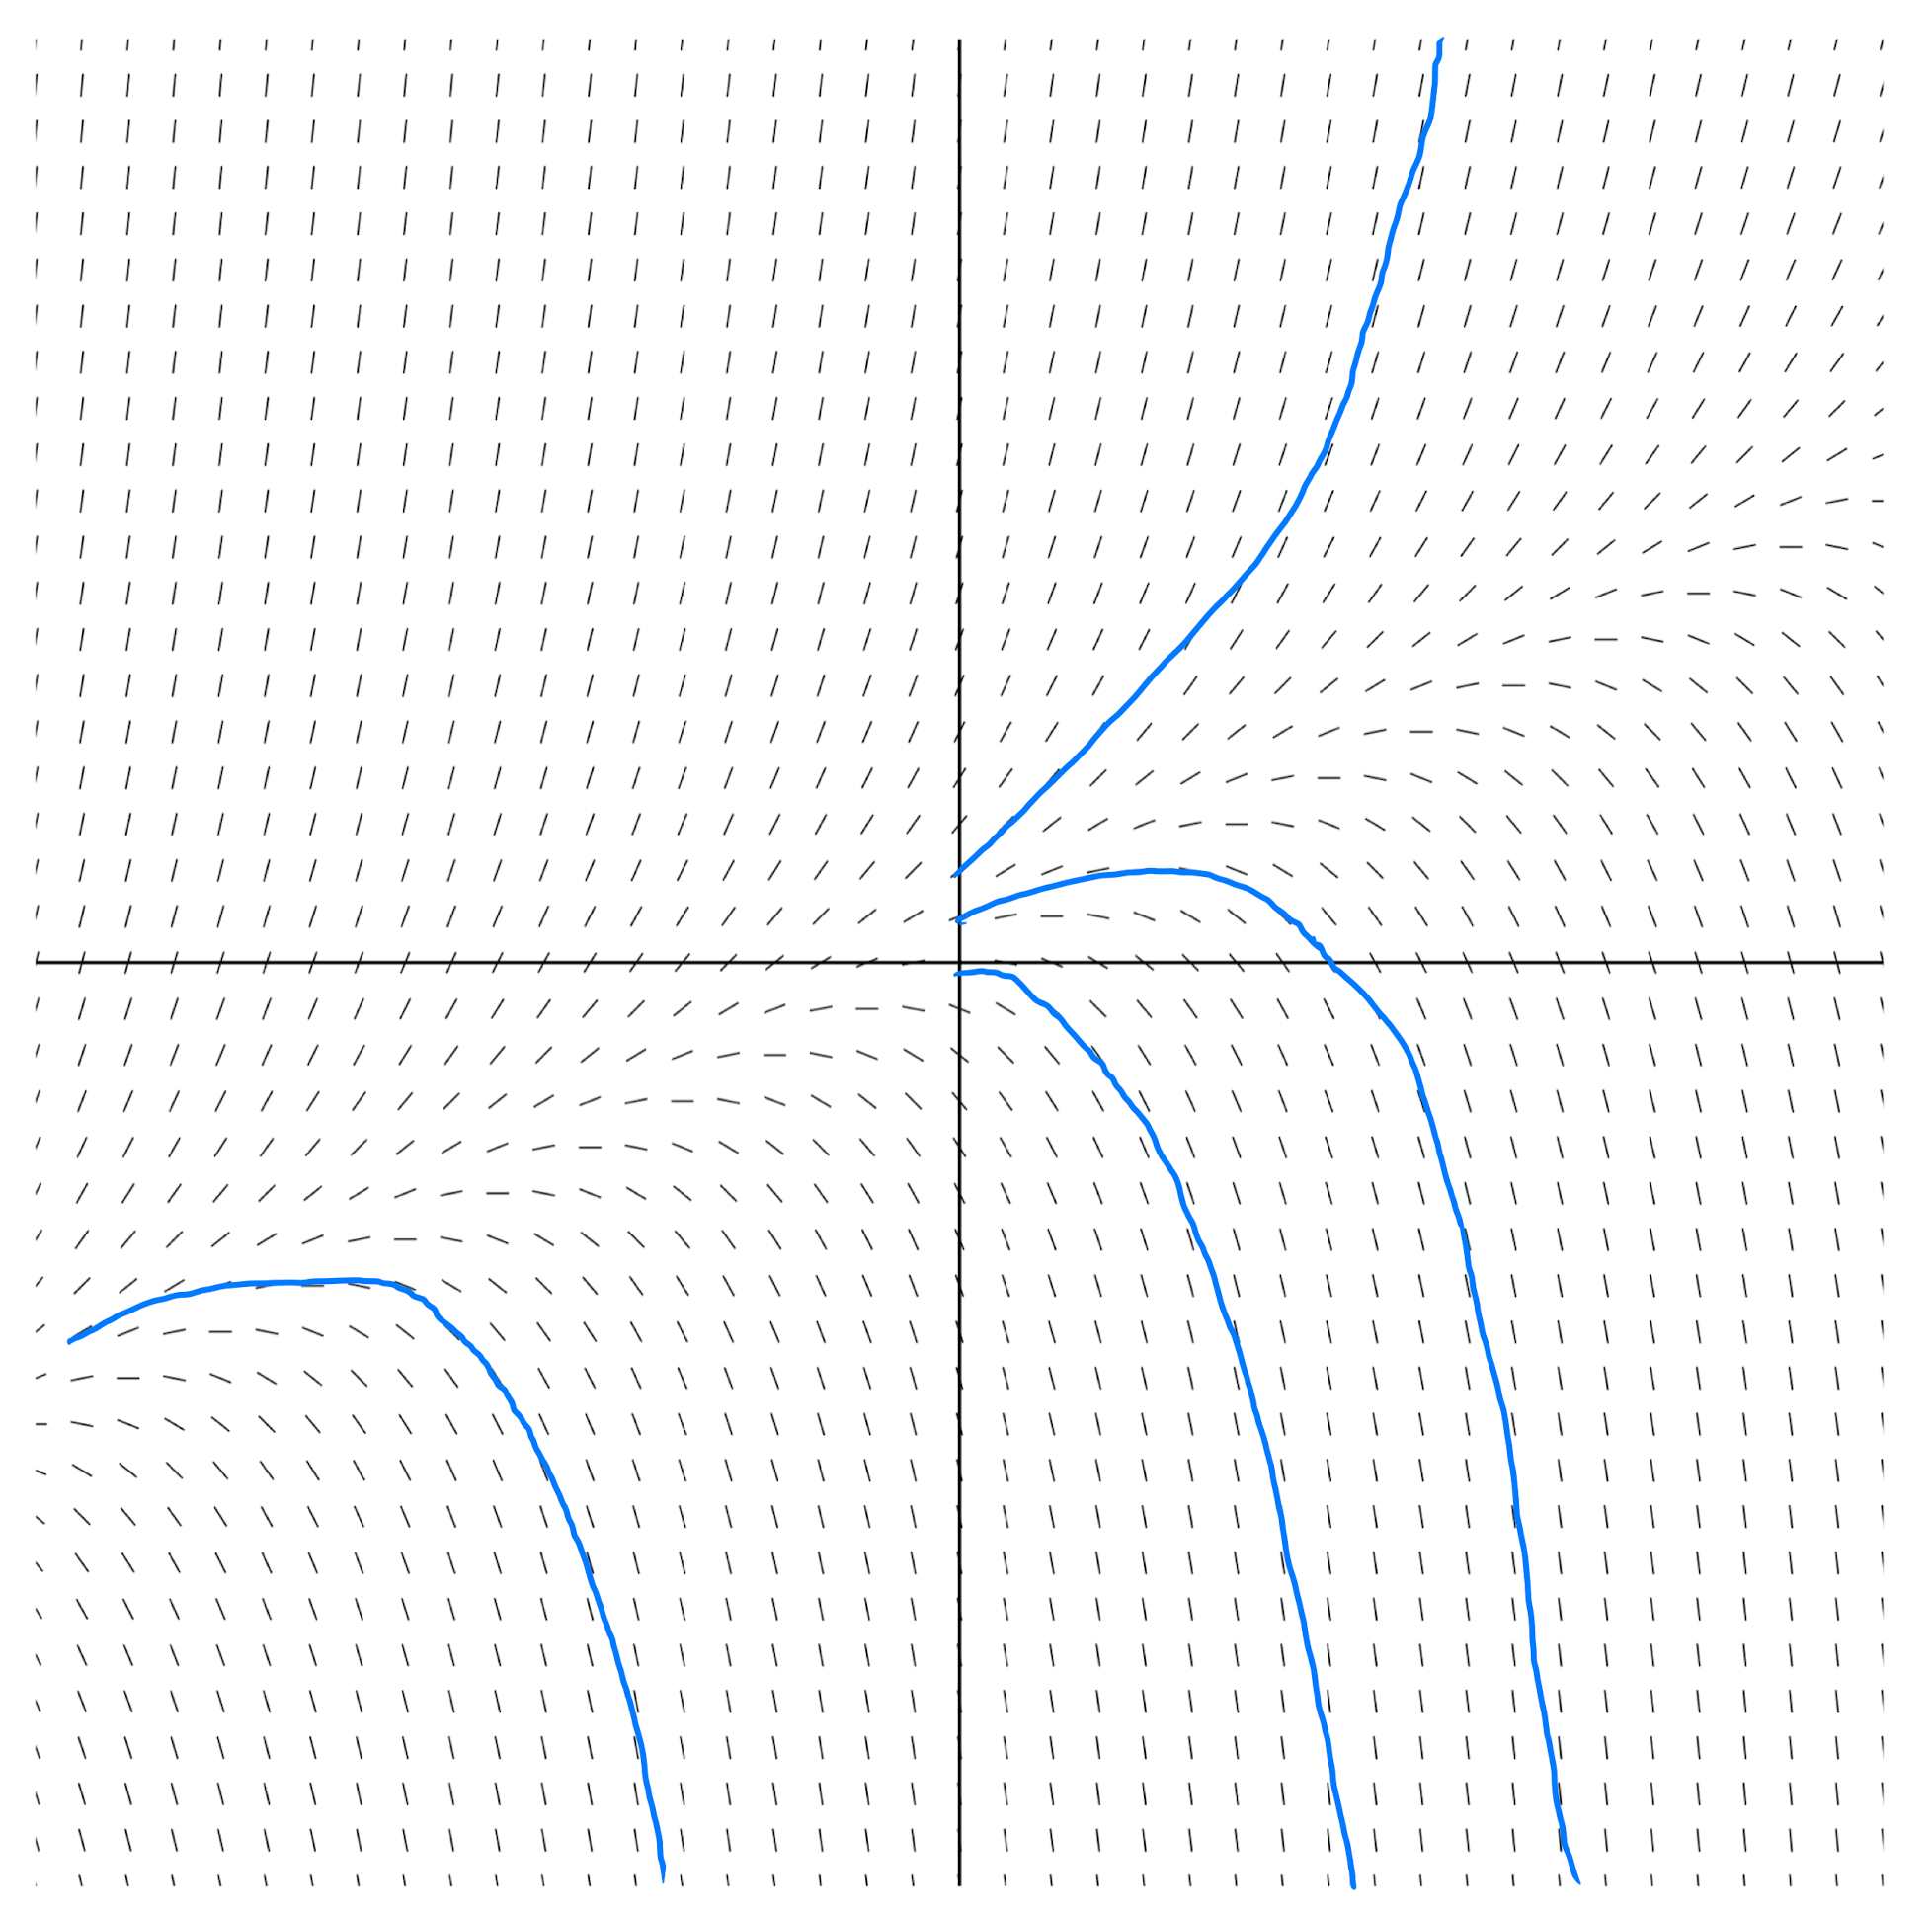
\includegraphics[width=10cm]{images/1_3_8.png}
\end{center}
For the solution with initial condition of $y(0) = 1/2$, the slope field suggests that the solution will increase without bound as $t$ increases.
%\begin{center}
%\begin{tikzpicture}
%%% Set the window for x and y values.
%\pgfmathsetmacro\xmin{-4};
%\pgfmathsetmacro\ymin{-4};
%\pgfmathsetmacro\xmax{4};
%\pgfmathsetmacro\ymax{4};
%%% Set the density of the slope field; a lower spacing gives a denser slope field.
%\pgfmathsetmacro\xspacing{0.2};
%\pgfmathsetmacro\yspacing{0.2};
%%% Set the length of the tangent lines: all lines of the slope field are drawn with this length. This should be less than both spacing numbers above for a neat slope field.
%\pgfmathsetmacro\length{0.1};
%%% Define the slope at (\x,\y) as a function f of \x and \y. Here, #1 is \x and #2 is \y. The function should be defined within \pgfmathparse{ }.
%\pgfmathdeclarefunction{f}{2}{\pgfmathparse{-1*(#1) + 1*(#1) + 3*(#2)*(1-(#2))}};
%
%%% This block generates the slope field.
%%% Restrict drawing to the confines of the specified rectangle.
%\clip (\xmin,\ymin) rectangle (\xmax,\ymax);
%%% Draw the axes.
%\draw (\xmin,0) -- (\xmax,0);
%\draw (0,\ymin) -- (0,\ymax);
%%% Some calculations (since we cannot do arithmetic inside a list).
%\pgfmathsetmacro\xnext{\xmin+\xspacing};
%\pgfmathsetmacro\ynext{\ymin+\yspacing};
%%% Loop to draw the tangent lines.
%\foreach \x in {\xmin,\xnext, ..., \xmax}{ \foreach \y in {\ymin, \ynext, ..., \ymax}{
%%% Calculate slope at (\x,\y).
%\pgfmathsetmacro\slope{f(\x,\y)};
%\begin{scope}
%%% Cut the drawing down to the circle of radius 0.5*\length centered at (\x,\y).
%\clip (\x,\y) circle ({0.5*\length});
%%% Draw tangent lines of length at least \length, with midpoint (\x,\y).
%\draw[very thin] ({\x - 0.5*\length}, {\y - 0.5*\slope*\length}) -- ({\x + 0.5*\length}, {\y + 0.5*\slope*\length});
%\end{scope}
%}
%}
%
%\end{tikzpicture}
%\end{center}
%\begin{center}
%  \begin{tikzpicture}[scale=2]
%    \begin{axis}[
%      view     = {0}{90},
%      domain   = -4:4,
%      y domain = -4:4,
%      samples  = 21,
%      xmax     = 4,
%      ymax     = 4,
%      ymin=-4,
%      xmin=-4,
%      axis lines*=center,
%      xtick={-4,-3,-2,-1,0,1,2,3,4},
%ytick={-4,-3,-2,-1,0,1,2,3,4},
%    ]
%    \addplot3 [gray, quiver={u={1/sqrt(1 + (2*y-x)^2)}, v={(2*y - x)/sqrt(1 + (2*y-x)^2)}, scale arrows=0.3,
%               every arrow/.append style={line width=0.5pt*\pgfplotspointmetatransformed/1000}}] (x,y,0);
%   % \addplot [thick, red] table [x=x, y=y] {\loadedtable};
%  \end{axis}
%  \end{tikzpicture}
%\end{center}
%\begin{align*}
%  \frac{dy}{dt} &= 2y-t
%\end{align*}
\subsection{1.3, Problem 12}%
\begin{enumerate}[(a)]
  \item $f(t,y)$ is equal to zero when $y = 2$.
  \item We are able to sketch the equilibrium solution of $y(t) = 2$.
  \item This does not tell us any other information for when $y(0) \neq 2$.
\end{enumerate}
\subsection{1.3, Problem 13}%
\begin{center}
  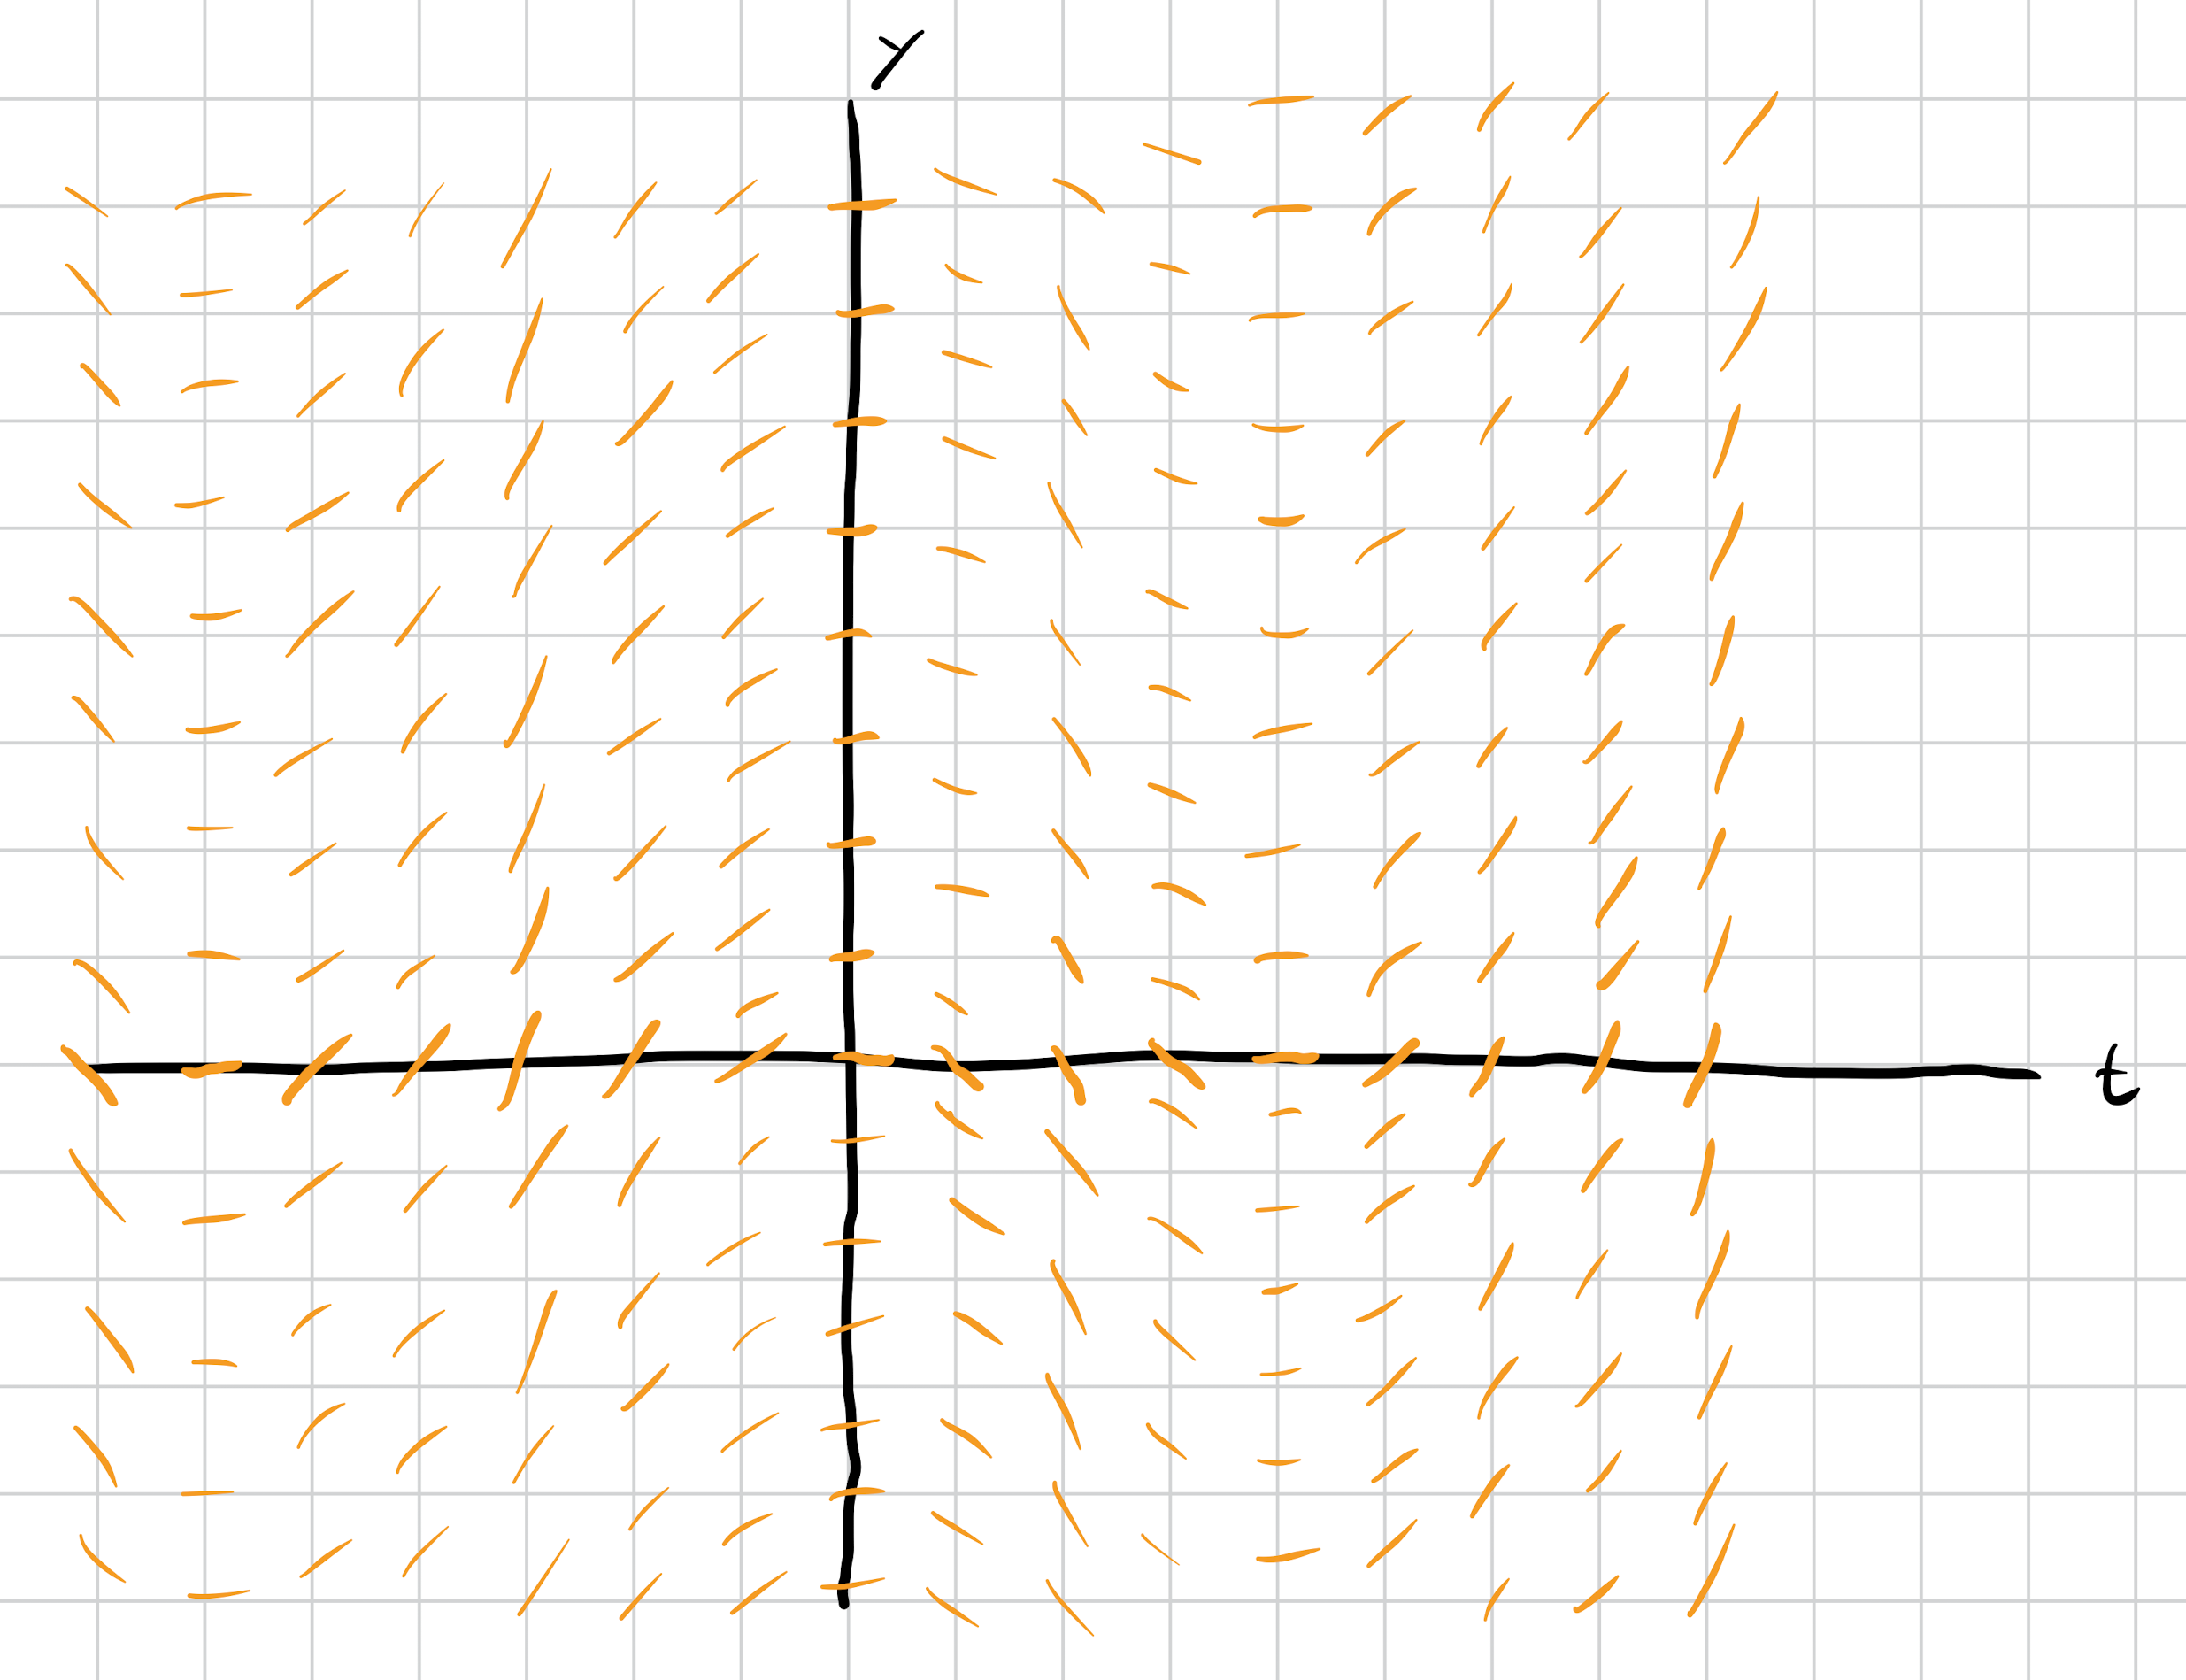
\includegraphics[width=10cm]{images/1_3_13.png}
\end{center}
\subsection{1.3, Problem 14}%
\begin{center}
  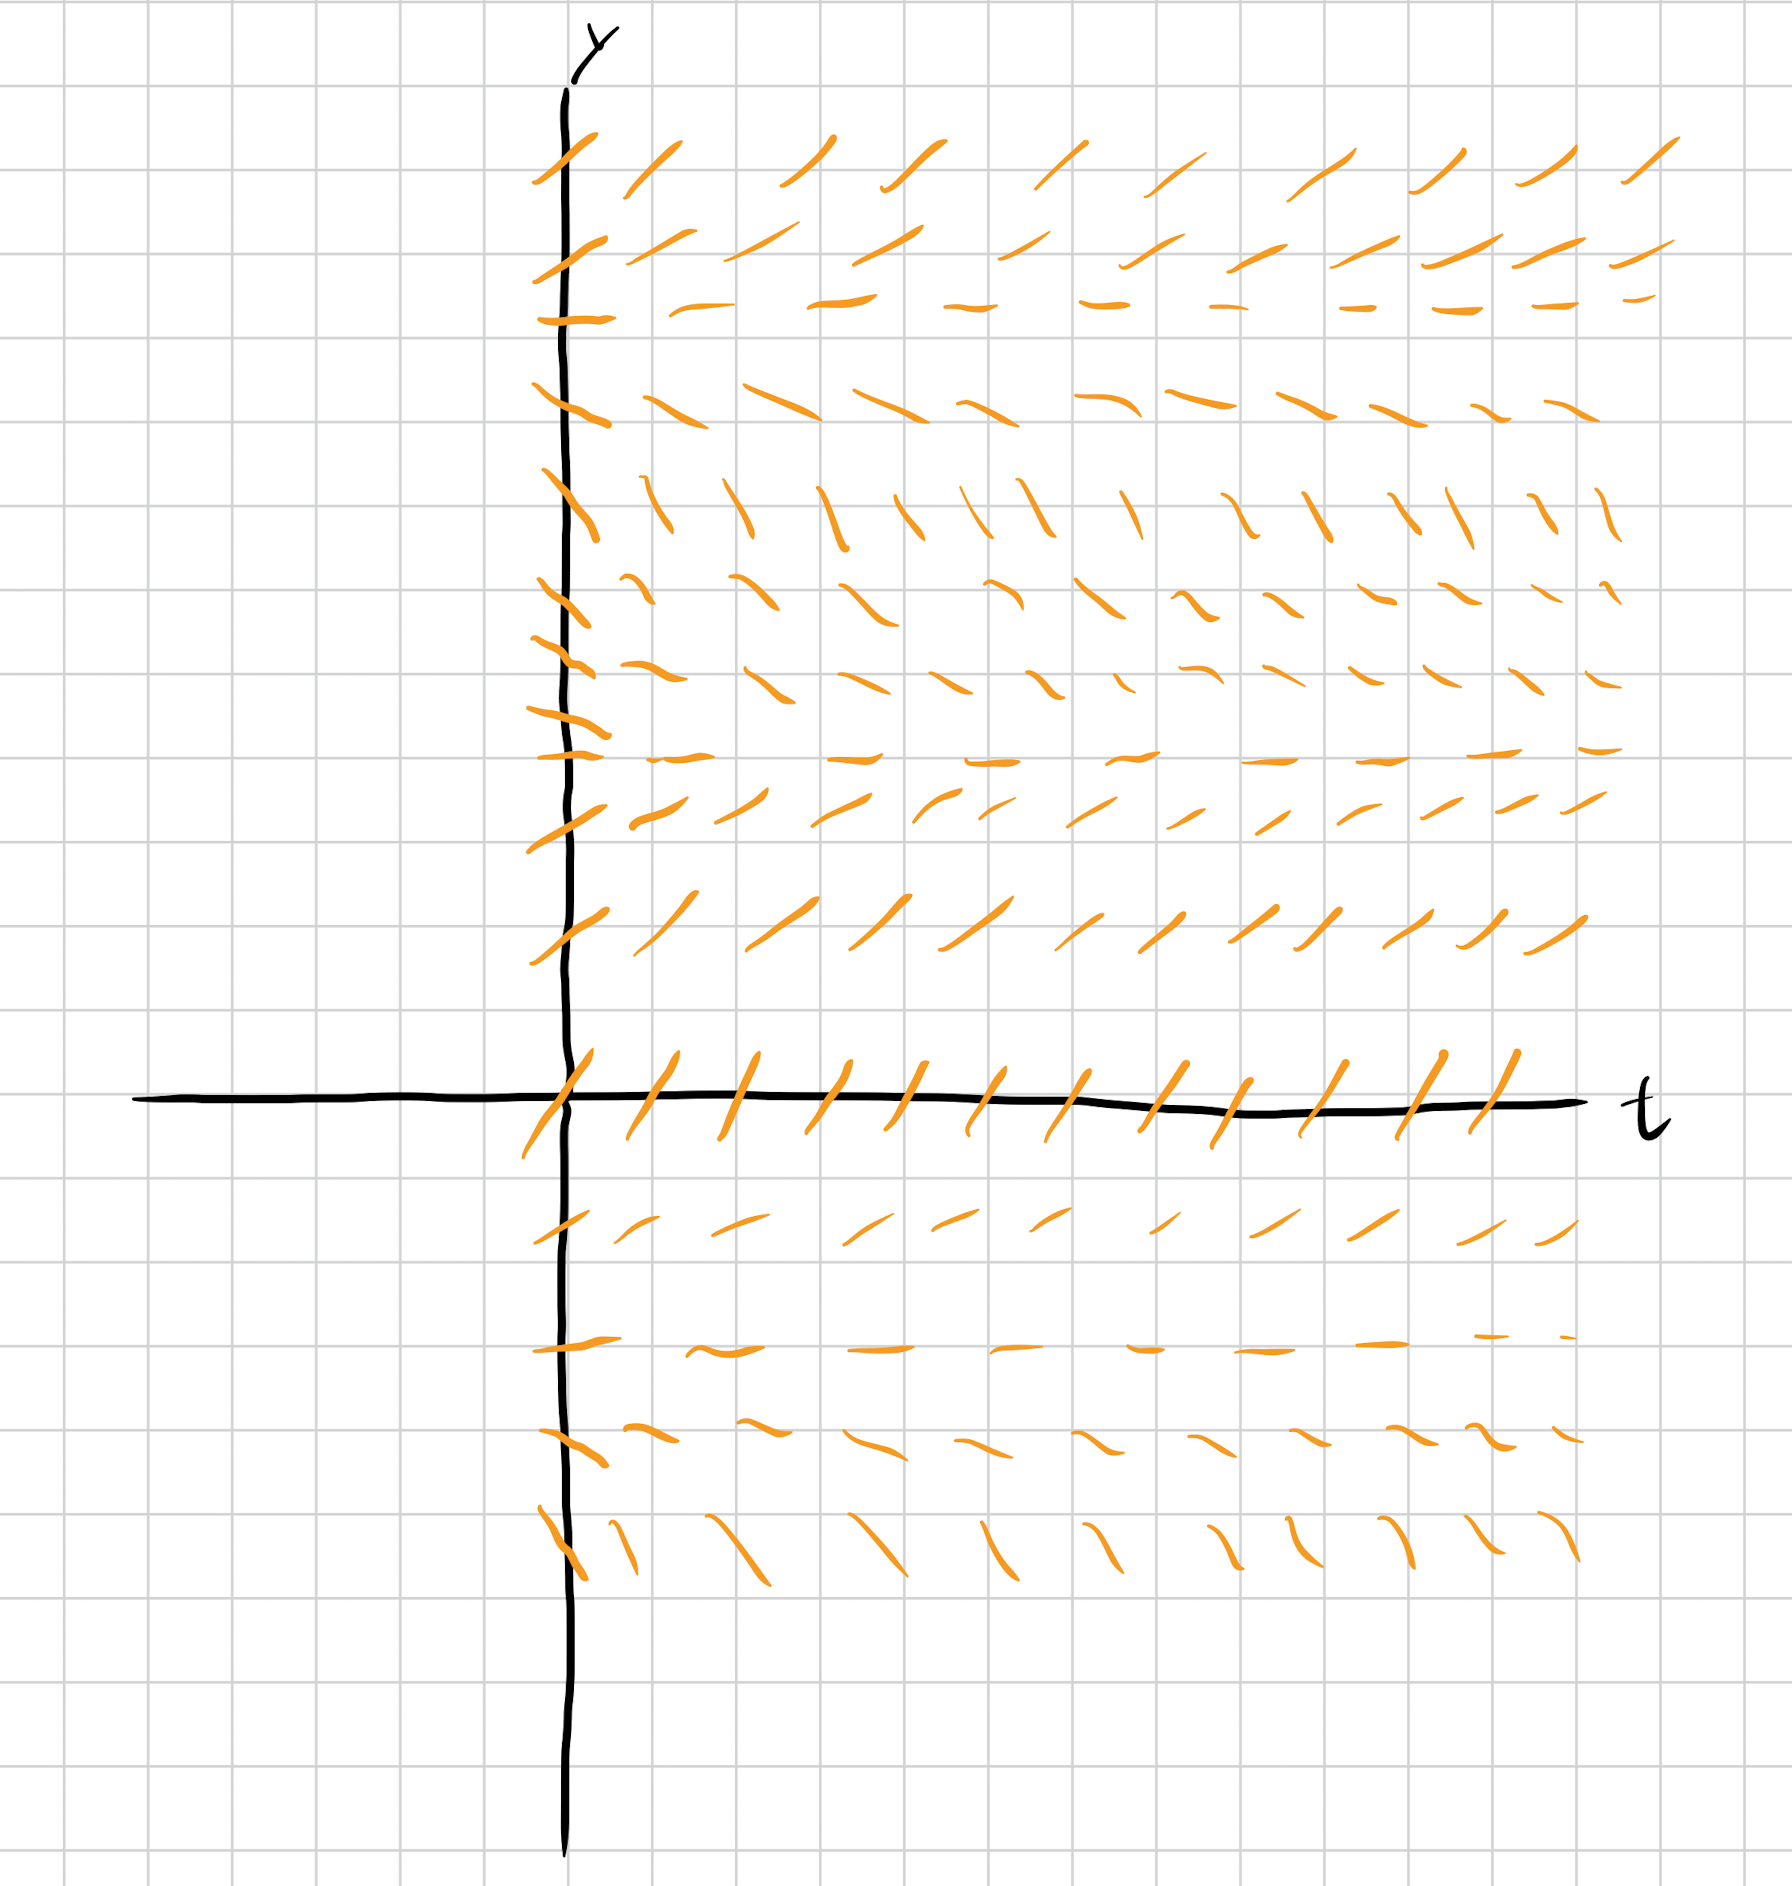
\includegraphics[width=10cm]{images/1_3_14.png}
\end{center}
\subsection{1.3, Problem 16}%
\begin{enumerate}[(a)]
  \item This slope field is for equation, (iii), as the slopes are purely dependent on $y$ and equal to zero at $y=0$, $y=-1$. Additionally, the slope is negative for all $y < -1$, which implies that it cannot be of the form $y^2$.
  \item This slope field is for equation (viii), as it reaches slop $0$ at $\pm \sqrt{2}$, and for $t > \sqrt{2}$, the slope is positive.
  \item This slope field is for equation (v), as it has slope zero at $y=0$ and $y=-1$ and has $t$-dependence that changes with sign.
  \item This slope field is for equation (vi), as it has slope zero at $y=-1$ and $t$-dependence with positive sign (i.e., always negative when $y + 1 < 0$).
\end{enumerate}
\end{document}
